\chapter{Algoritmos de Ordenação}
\chaplabel{sorting}

Este capítulo discute algoritmos para classificar um conjunto de #n# itens.
Isso pode parecer um tópico estranho para um livro sobre estruturas de dados, mas
existem várias boas razões para incluí-lo aqui. O motivo mais óbvio é que dois desses algoritmos de classificação (quicksort e heap-sort)
estão intimamente relacionados com duas das estruturas de dados que já estudamos (árvores aleatórias de busca binárias e pilhas, respectivamente).

A primeira parte deste capítulo discute algoritmos que classificam usando apenas comparações e apresenta três algoritmos que são executados em um tempo de $O(#n#\log #n#)$. Como se verifica, os três algoritmos são assintoticamente ótimos; nenhum algoritmo que use apenas comparações pode evitar de fazer aproximadamente $#n#\log #n#$ comparações no pior caso e até mesmo no caso médio.

Antes de continuar, devemos notar que qualquer das implementações de #SSet# ou de #Fila# de prioridades apresentadas em capítulos anteriores também podem ser usadas para obter um algoritmo de classificação com tempo $O(#n#\log #n#)$. Por exemplo, podemos classificar #n# itens executando #n# operações #add(x)# seguidas de #n#  operações #remove()# em #BinaryHeap# ou #MeldableHeap#. Alternativamente, podemos usar as #n# operações #add(x)# em qualquer uma das estruturas de dados da árvore de pesquisa binária e, em seguida, executar uma travessia em ordem (\excref{tree-traversal}) para extrair os elementos ordenados. No entanto, em ambos os casos, temos um alto custo para construir uma estrutura que nunca é totalmente utilizada. A classificação é um problema tão importante que vale a pena desenvolver métodos diretos que sejam tão rápidos, simples e eficientes em termos de espaço quanto possível.

A segunda parte deste capítulo mostra que, se permitimos outras operações além de comparações, todas as possibilidades são possíveis. De fato, usando a indexação de array, é possível classificar um conjunto de #n# inteiros na faixa $\{0,\ldots,#n#^c-1\}$ em um tempo $O(c#n#)$.



\section{Ordenação Baseada em Comparações}

\index{ordenação baseada em comparação}%
\index{algoritmo de ordenação!baseada em comparação}%
Nesta seção, apresentamos três algoritmos de classificação: merge-sort, quicksort e heap-sort. Cada um desses algoritmos recebe um array de entrada #a# e classifica os elementos de #a# em ordem não decrescente em um tempo (esperado) de $O(#n#\log#n#)$. Esses algoritmos são todos \emph{baseados em comparação}.
\javaonly{O segundo argumento, #c#, é um #Comparator#
\index{Comparador@#Comparador#}%
que implementa
o método #compare(a,b)#
\index{compare@#compare(a,b)#}%
.} Esses algoritmos não se importam com o tipo de dados que estão sendo classificados; a única operação que eles fazem nos dados é comparações usando o método #compare(a,b)#. Lembre-se de \secref{sset}, que #compare(a,b)# retorna um valor negativo se $#a#<#b#$, um valor positivo se $#a#>#b#$ e zero se $#a#=#b#$.

\subsection{Merge-Sort}
\seclabel{merge-sort}

\index{merge-sort}%
O algoritmo \emph{merge-sort} é um exemplo clássico de divisão e conquista recursiva:
\index{dividir e conquistar}%
Se o comprimento de #a# for no máximo 1, então #a# já está classificado, então não fazemos nada. Caso contrário, dividimos #a# em duas metades, $#a0#=#a[0]#,\ldots,#a[n/2-1]#$ e $#a1#=#a[n/2]#,\ldots,#a[n-1]#$. Nós classificamos recursivamente #a0# e #a1#, e então mesclamos (o agora ordenado) #a0# e #a1# para obter nossa matriz totalmente ordenada #a#:
\javaimport{ods/Algorithms.mergeSort(a,c)}
\cppimport{ods/Algorithms.mergeSort(a)}
\pcodeimport{ods/Algorithms.mergeSort(a)}
Um exemplo é mostrado na \figref{merge-sort}.
\begin{figure}
  \begin{center}
    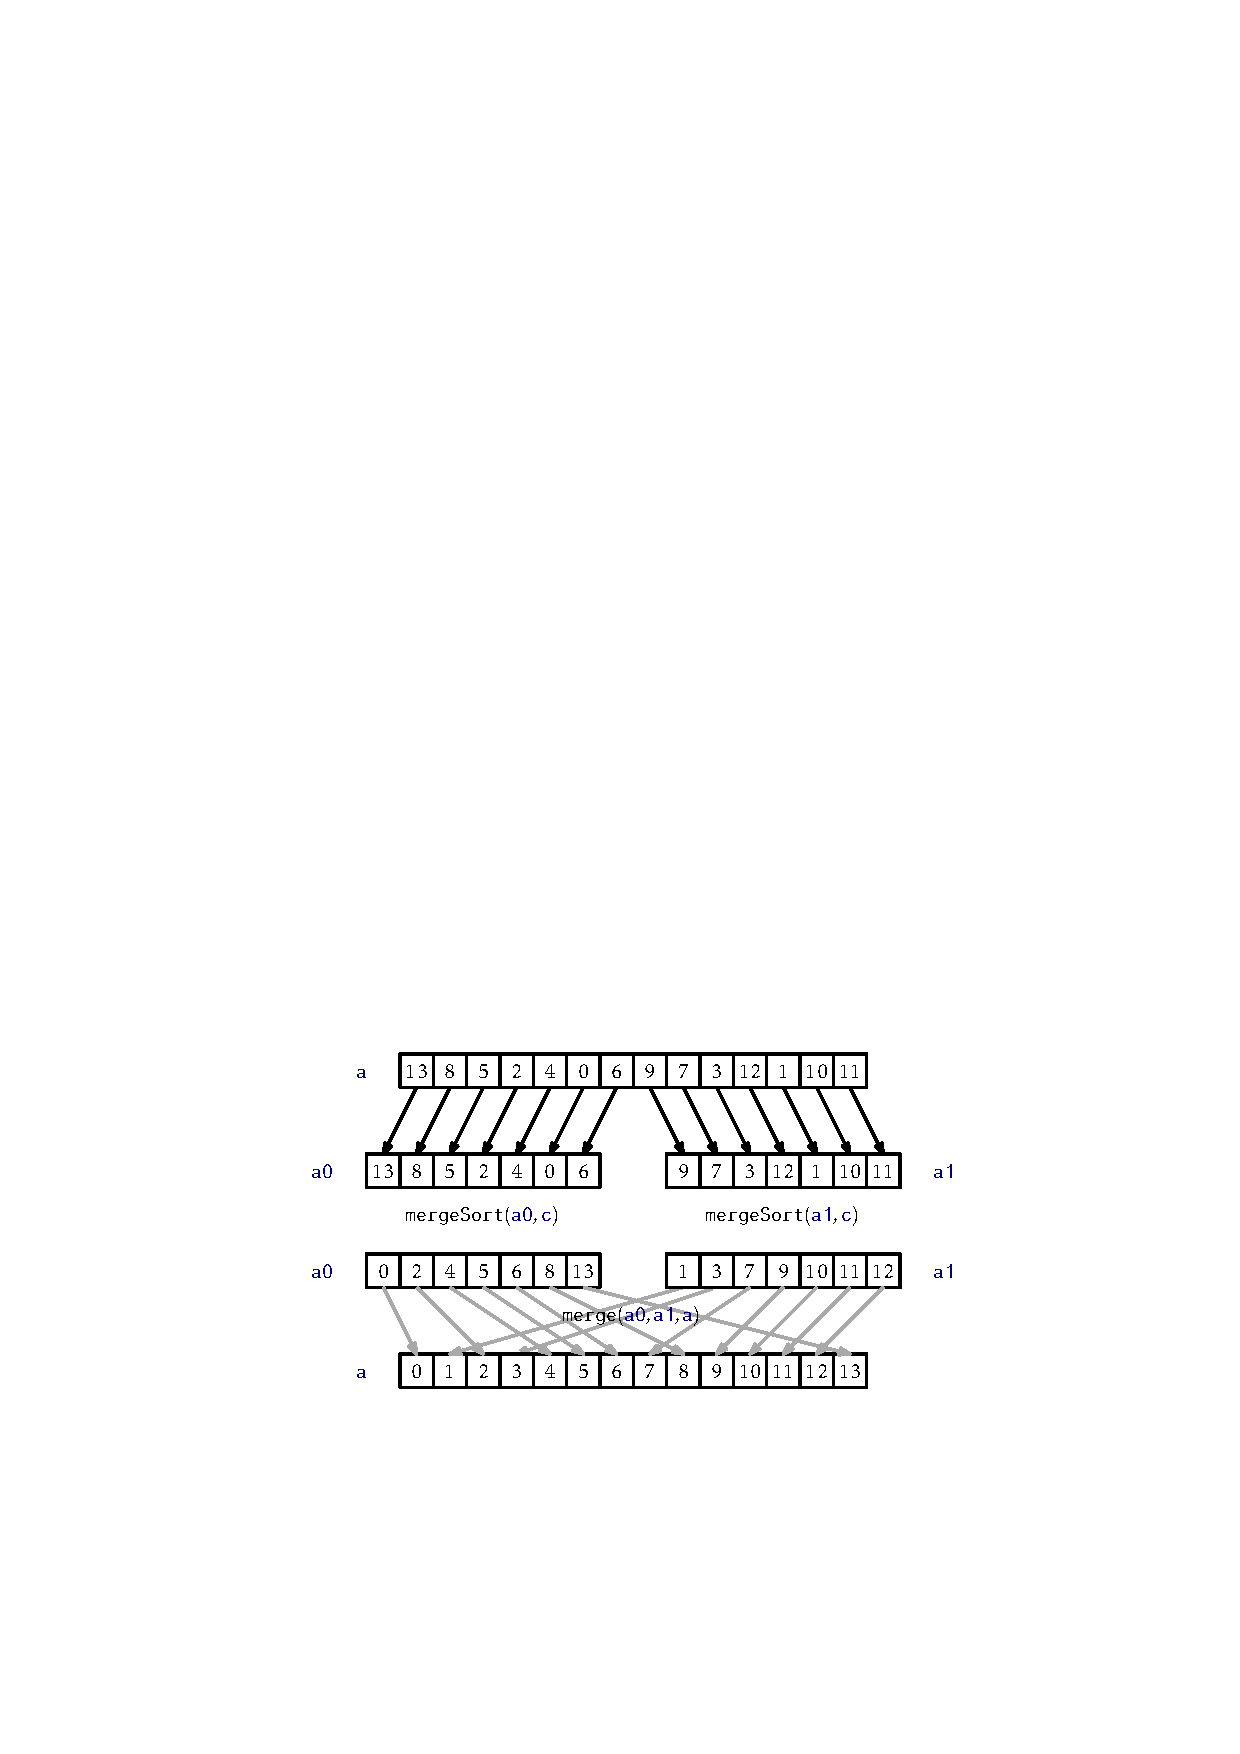
\includegraphics[width=\ScaleIfNeeded]{figs/mergesort}
  \end{center}
  \caption[Merge sort]{A execução de #mergeSort(a,c)#}
  \figlabel{merge-sort}
\end{figure}


Em comparação com a classificação, a mesclagem dos dois arrays classificados #a0# e #a1# é bastante fácil. Nós adicionamos elementos em #a# um por vez. Se #a0# ou #a1# estiver vazio, então adicionamos os próximos elementos do outro array (não vazio). Caso contrário, nós colocamos o mínimo do próximo elemento em #a0# e o próximo elemento em #a1# e o adicionamos a #a#:
\javaimport{ods/Algorithms.merge(a0,a1,a,c)}
\cppimport{ods/Algorithms.merge(a0,a1,a)}
\pcodeimport{ods/Algorithms.merge(a0,a1,a)}
Observe que o algoritmo #merge(a0,a1,a,c)# executa no máximo $#n#-1$ comparações antes de ficar sem elementos em um #a0# ou #a1#.

Para entender o tempo de execução do merge-sort, é mais fácil pensar nele em termos de sua árvore de recursão. Suponha agora que #n# é uma potência de dois, de modo que $#n#=2^{\log #n#}$ e $\log #n#$ é um número inteiro. Consulte \figref{mergesort-recursion}. Merge-sort transforma o problema de classificar #n# elementos em dois problemas, cada um dos elementos de classificação $#n#/2$. Estes dois subproblemas são então transformados em dois problemas cada, para um total de quatro subproblemas, cada um de tamanho $#n#/4$. Esses quatro subproblemas tornam-se oito subproblemas, cada um de tamanho $#n#/8$, e assim por diante. No final deste processo, os subproblemas $#n#/2$, cada um de tamanho dois, são convertidos em #n# problemas, cada um de tamanho um. Para cada subproblema de tamanho $#n#/2^{i}$, o tempo gasto para mesclar e copiar dados é $O(#n#/2^i)$. Uma vez que existem $2^i$ subproblemas de tamanho $#n#/2^i$, o tempo total gasto trabalhando em problemas de tamanho $2^i$, sem contar chamadas recursivas, é
\[
       2^i\times O(#n#/2^i) = O(#n#) \enspace .
\]
Portanto, a quantidade total de tempo tomado por merge-sort é
\[
   \sum_{i=0}^{\log #n#} O(#n#) = O(#n#\log #n#) \enspace .
\]

\begin{figure}
  \begin{center}
    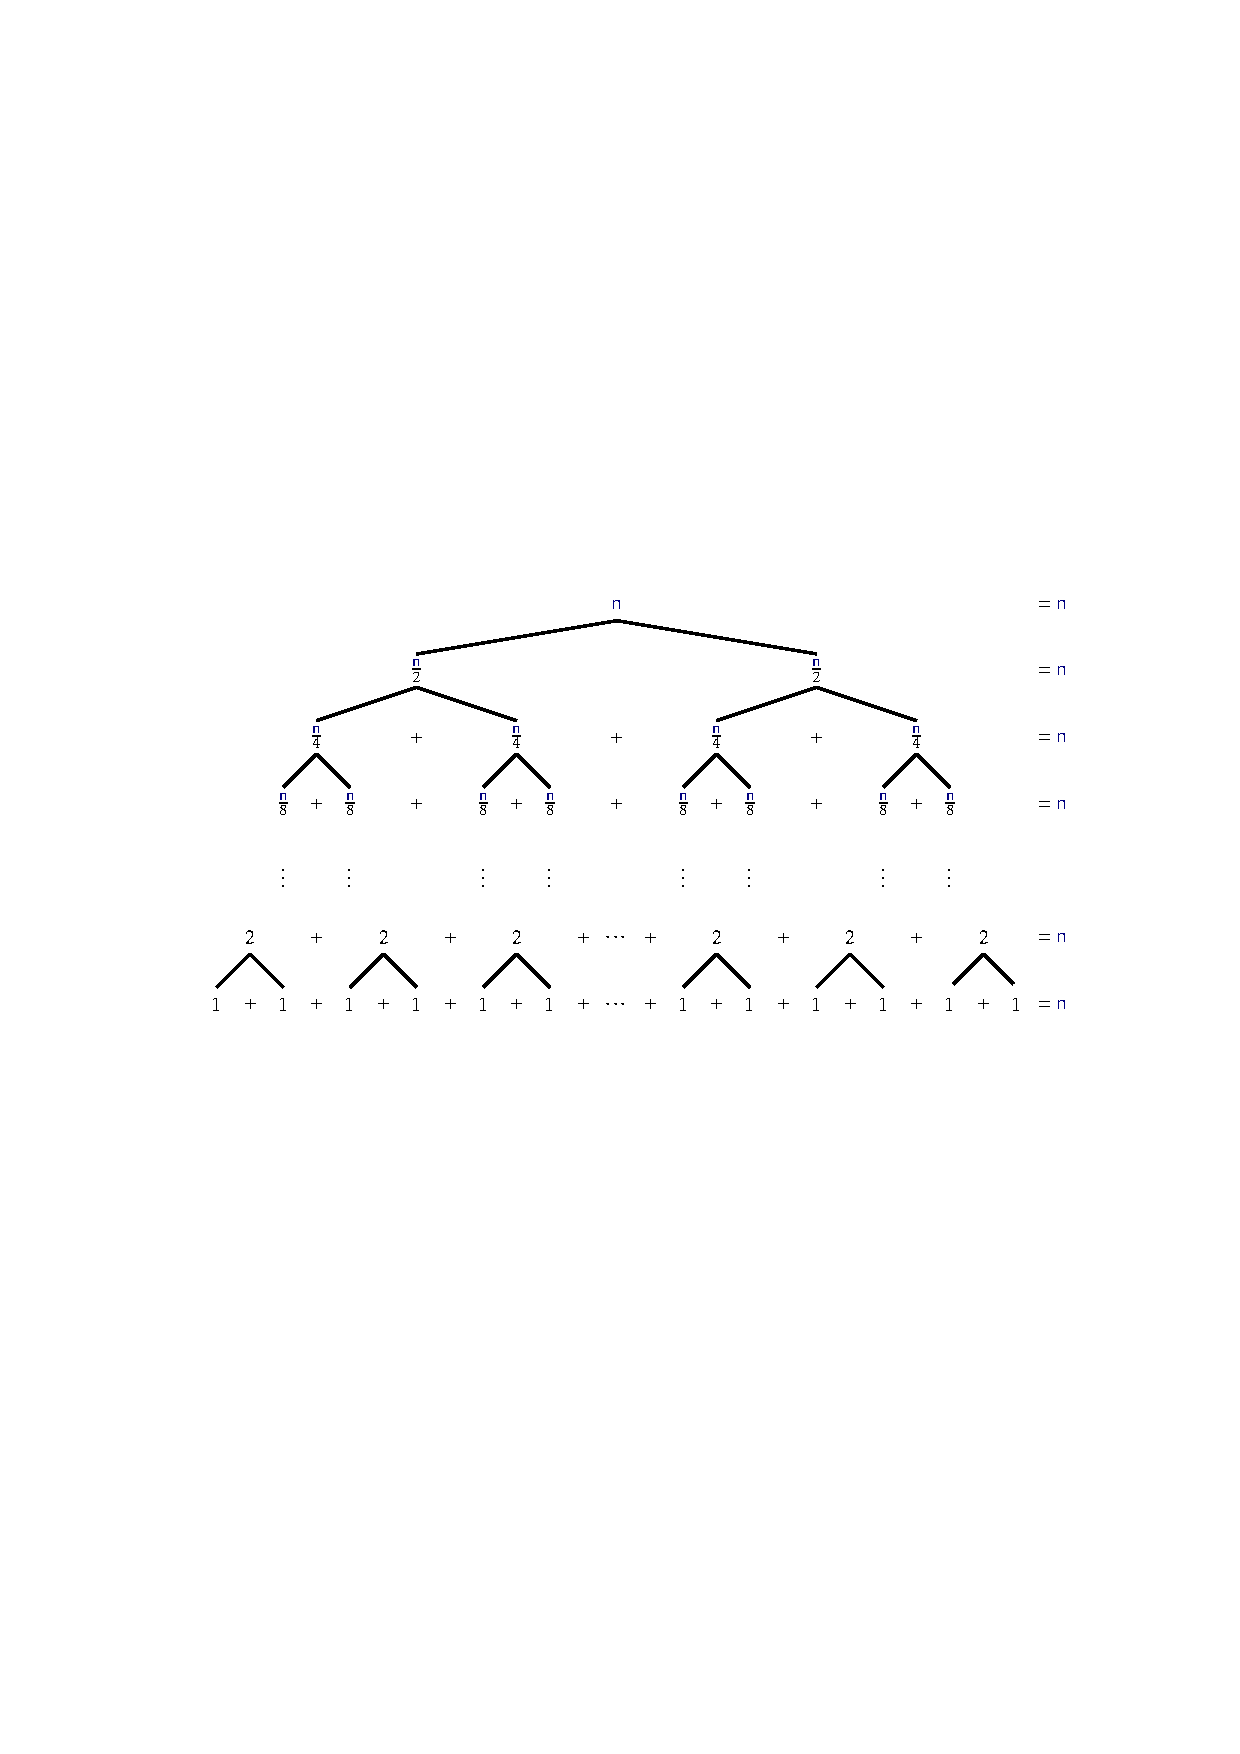
\includegraphics[width=\ScaleIfNeeded]{figs/mergesort-recursion}
    \caption{A árvore de recursão de merge-sort.}
    \figlabel{mergesort-recursion}
  \end{center}
\end{figure}

A prova do seguinte teorema baseia-se na análise anterior, mas tem que ser um pouco mais cuidadosa para lidar com os casos em que #n# não é uma potência de 2.
\begin{thm}
  O algoritmo \javaonly{#mergeSort(a,c)#}\cpponly{mergeSort(a)}\pcodeonly{merge\_sort(a)} executa em um tempo $O(#n#\log #n#)$ e faz
  no máximo $#n#\log #n#$ comparações.
\end{thm}

\begin{proof}
A prova é por indução em $#n#$. O caso base, em que $#n#=1$, é trivial; quando apresentado com uma matriz de comprimento 0 ou 1, o algoritmo simplesmente retorna sem realizar comparações.

A combinação de duas listas ordenadas do comprimento total $#n#$ requer no máximo $#n#-1$ comparações. Faça $C(#n#)$ indicar o número máximo de comparações realizadas por #mergeSort(a,c)# em um array #a# de comprimento #n#. Se $#n#$ for uniforme, então aplicamos a hipótese indutiva aos dois subproblemas e obtemos
\begin{align*}
  C(#n#) 
  &\le #n#-1 + 2C(#n#/2) \\
  &\le #n#-1 + 2((#n#/2)\log(#n#/2)) \\
  &= #n#-1 + #n#\log(#n#/2) \\
  &= #n#-1 + #n#\log #n#-#n# \\
  &< #n#\log #n# \enspace .
\end{align*}
O caso em que $#n#$ é ímpar é um pouco mais complicado. Para este caso, usamos duas desigualdades que são fáceis de verificar:
\begin{equation}
  \log(x+1) \le \log(x) + 1 \enspace , \eqlabel{log-ineq-a}
\end{equation}
for all $x\ge 1$ e
\begin{equation}
  \log(x+1/2) + \log(x-1/2) \le 2\log(x) \enspace , \eqlabel{log-ineq-b}
\end{equation}
para todo $x\ge 1/2$.  A desigualdade~\myeqref{log-ineq-a} vem do fato de que $\log(x)+1=\log(2x)$ enquanto \myeqref{log-ineq-b} decorre do fato de que $\log$ é uma função côncava. Com essas ferramentas na mão, temos, para o #n# ímpar,
\begin{align*}
  C(#n#) 
  &\le #n#-1 + C(\lceil #n#/2 \rceil) + C(\lfloor #n#/2 \rfloor) \\
  &\le #n#-1 + \lceil #n#/2 \rceil\log \lceil #n#/2 \rceil 
           + \lfloor #n#/2 \rfloor\log \lfloor #n#/2 \rfloor \\
  &= #n#-1 + (#n#/2 + 1/2)\log (#n#/2+1/2) 
           + (#n#/2 - 1/2) \log (#n#/2-1/2) \\
  &\le #n#-1 + #n#\log(#n#/2) + (1/2)(\log (#n#/2+1/2) 
           - \log (#n#/2-1/2)) \\
  &\le #n#-1 + #n#\log(#n#/2) + 1/2 \\
  &< #n# + #n#\log(#n#/2) \\
  &= #n# + #n#(\log#n#-1) \\
  &= #n#\log#n# \enspace . \qedhere
\end{align*} 
\end{proof}

\subsection{Quicksort}

\index{quicksort}%
O algoritmo \emph{quicksort} é outro algoritmo clássico de divisão e conquista. Ao contrário do merge-sort, que se funde depois de resolver os dois subproblemas, o quicksort faz todo o seu trabalho antecipadamente.

Quicksort é simples de descrever: escolha um elemento aleatório \emph{pivô}, 
\index{elemento pivô}% 
#x#, de #a#; divida #a# no conjunto de elementos menores que #x#, o conjunto de elementos iguais a #x# e o conjunto de elementos maior que #x#; e, finalmente, ordene recursivamente o primeiro e o terceiro conjunto nesta partição. Um exemplo é mostrado na \figref{quicksort}.
\javaimport{ods/Algorithms.quickSort(a,c).quickSort(a,i,n,c)}
\cppimport{ods/Algorithms.quickSort(a).quickSort(a,i,n)}
\pcodeimport{ods/Algorithms.quickSort(a).quickSort(a,i,n)}
\begin{figure}
  \begin{center}
    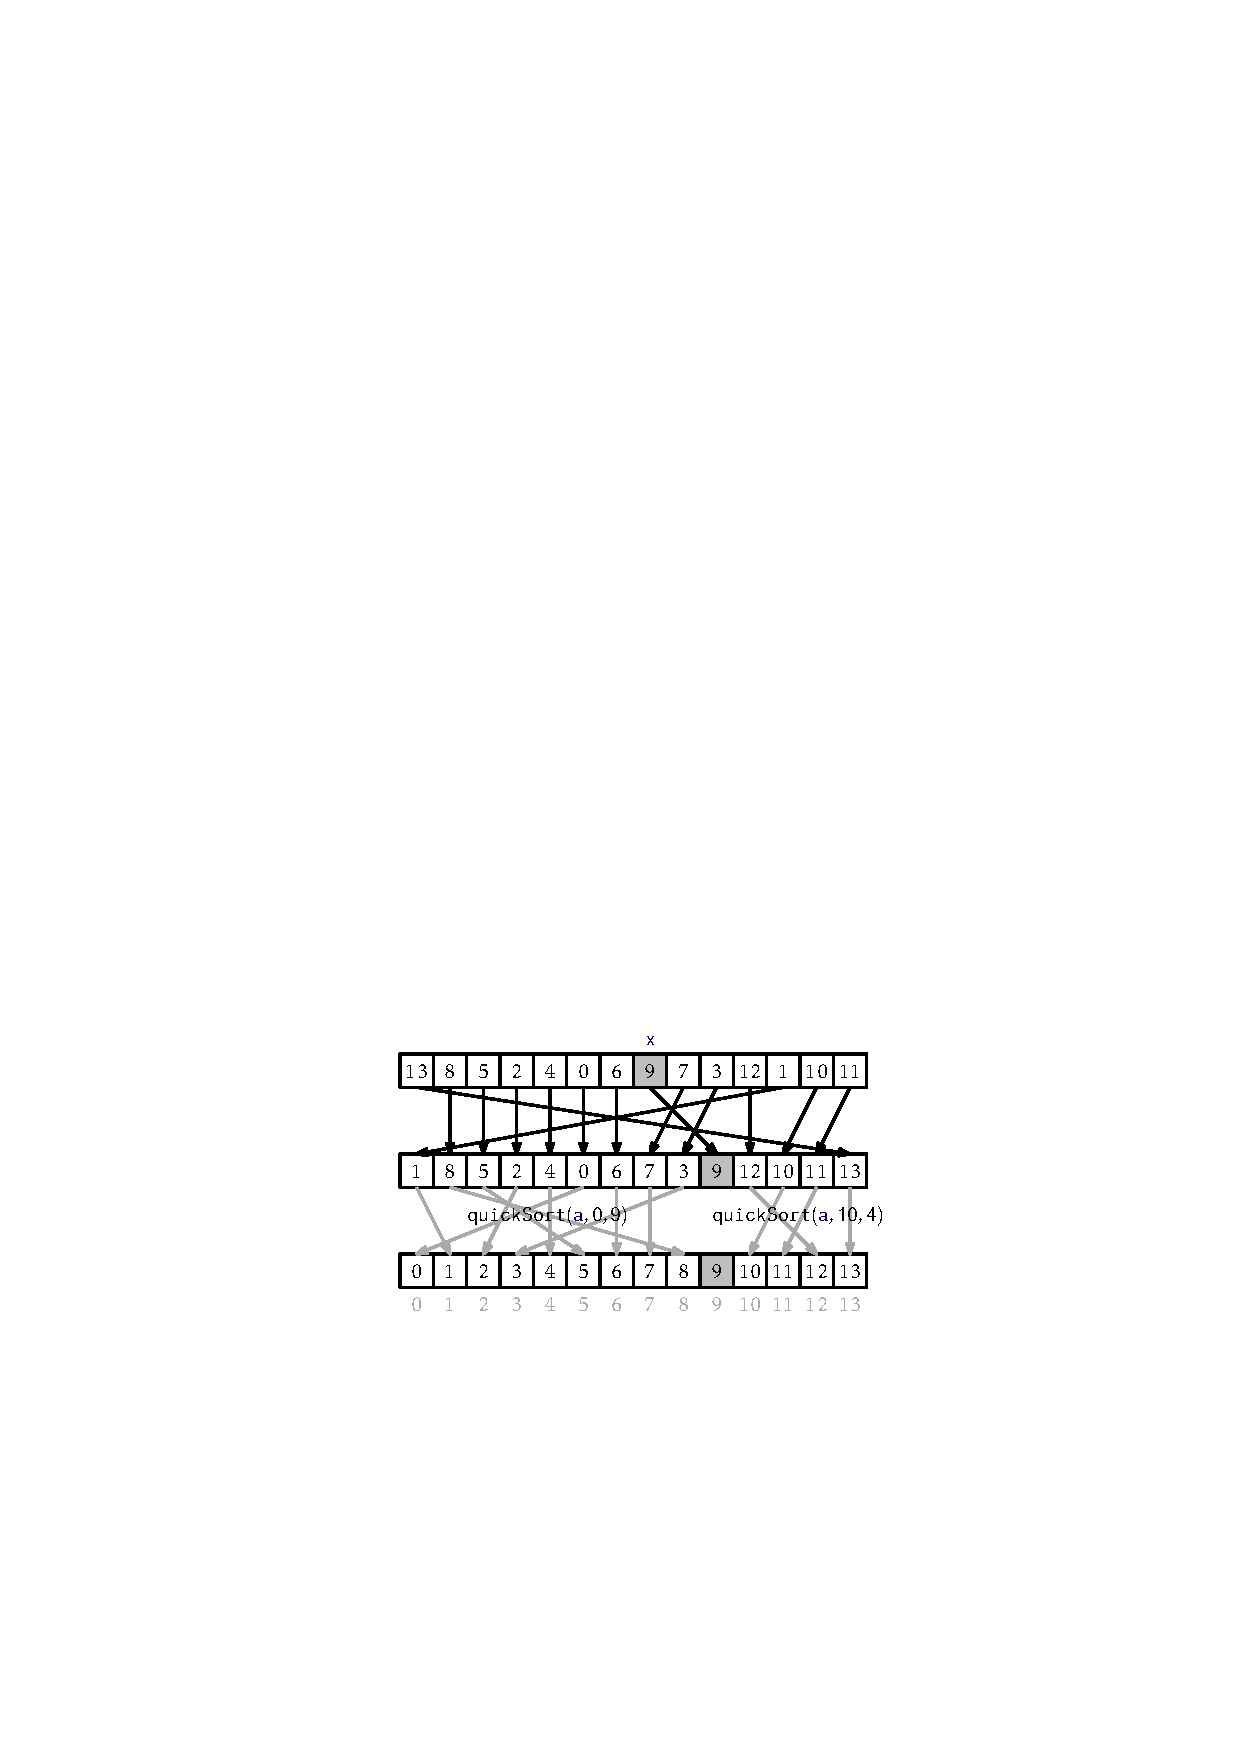
\includegraphics[scale=0.90909]{figs/quicksort}
    \caption[Quicksort]{Um exemplo da execução de \javaonly{#quickSort(a,0,14,c)#}\cpponly{#quickSort(a,0,14)#}\pcodeonly{#quickSort(a,0,14)#}}
    \figlabel{quicksort}
  \end{center}
\end{figure}
Tudo isso é feito no próprio array, em vez de fazer as cópias de subarrays serem ordenadas, o método #quickSort(a,i,n,c)# apenas ordena o subarray $#a[i]#,\ldots,#a[i + n-1]#$. Inicialmente, esse método é invocado com os argumentos 
#quickSort(a,0,a.length,c)#.

No coração do algoritmo quicksort está o algoritmo de particionamento no local. Este algoritmo, sem usar espaço extra, troca elementos em #a# e calcula índices #p# e #q# de modo que
\[
   #a[i]# \begin{cases} 
         {}< #x# & \text{if $0\le #i#\le #p#$} \\
         {}= #x# & \text{if $#p#< #i# < #q#$} \\
         {}> #x# & \text{if $#q#\le #i# \le #n#-1$}
     \end{cases}
\]
Este particionamento, que é feito pelo loop #while# no código, funciona aumentando iterativamente #p# e diminuindo #q# enquanto mantém a primeira e a última dessas condições. Em cada etapa, o elemento na posição #j# é movido ou para a frente, ou à esquerda de onde está ou movido para trás. Nos dois primeiros casos, #j# é incrementado, enquanto no último caso, #j# não é incrementado, pois o novo elemento na posição # j # ainda não foi processado.

O algoritmo quicksort está fortemente relacionado às árvores de pesquisa binária aleatórias estudadas em \secref{rbst}. De fato, se a entrada para quicksort consiste em #n# elementos distintos, a árvore de recursão de quicksort é uma árvore de pesquisa binária aleatória. Para ver isso, lembre-se de que ao construir uma árvore de pesquisa binária aleatória, a primeira coisa que fazemos é escolher um elemento aleatório #x# e torná-lo a raiz da árvore. Depois disso, cada elemento será eventualmente comparado com #x#, com elementos menores indo para a subárvore esquerda e elementos maiores para a direita.

Em quicksort, selecionamos um elemento aleatório #x# e comparamos imediatamente tudo com #x#, colocando os elementos menores no início do array e elementos maiores no final do array. Quicksort, em seguida, classifica recursivamente o início do array e o fim do array, enquanto a árvore de pesquisa binária aleatória insere recursivamente elementos menores na subárvore da esquerda dos elementos raiz e maiores na subárvore direita da raiz.

A correspondência acima entre árvores de pesquisa binárias aleatórias e quicksort significa que podemos traduzir \lemref{rbs} para uma declaração sobre quicksort:

\begin{lem}\lemlabel{quicksort}
	Quando o quicksort é chamado para ordenar um array contendo os inteiros $0,\ldots,#n#-1$, o número esperado de vezes que o elemento #i# é comparado a um elemento de pivô é no máximo $H_{#i#+1} + H_{#n#-#i#}$.
\end{lem}

Uma pequena soma de números harmônicos nos dá o seguinte teorema sobre o tempo de execução do quicksort:

\begin{thm}\thmlabel{quicksort-i}
	Quando o quicksort é chamado para ordenar uma matriz contendo #n# elementos distintos, o número esperado de comparações realizadas é no máximo
  $2#n#\ln #n# + O(#n#)$.
\end{thm}

\begin{proof}
Seja $T$ o número de comparações realizadas pelo quicksort ao classificar #n# elementos distintos. Usando \lemref{quicksort} e a linearidade de expectativa, temos:
\begin{align*}
  \E[T] &= \sum_{i=0}^{#n#-1}(H_{#i#+1}+H_{#n#-#i#}) \\ 
        &= 2\sum_{i=1}^{#n#}H_i \\ 
        &\le 2\sum_{i=1}^{#n#}H_{#n#} \\ 
        &\le 2#n#\ln#n# + 2#n# = 2#n#\ln #n# + O(#n#) \qedhere
\end{align*}
\end{proof}

\thmref{quicksort} descreve o caso em que os elementos que estão sendo classificados são todos distintos. Quando o array de entrada, #a#, contém elementos duplicados, o tempo de execução esperado do quicksort não é pior e pode ser ainda melhor; sempre que um elemento duplicado #x# é escolhido como um pivô, todas as ocorrências de #x# são agrupadas e não participam de nenhum dos dois subproblemas.

\begin{thm}\thmlabel{quicksort}
	O método \javaonly{#quickSort(a,c)#} \cpponly{#quickSort(a)#} \pcodeonly{#quickSort(a,c)#} é executado em um tempo esperado de $O(#n#\log #n#)$ e o número esperado de comparações que executam são no máximo
  $2#n#\ln #n# +O(#n#)$.
\end{thm}

\subsection{Heap-sort}
\seclabel{heapsort}

\index{heap-sort}%
O algoritmo \emph{heap-sort} é outro algoritmo de classificação local. O heap-sort usa os heaps binários discutidos em \secref{binaryheap}. Lembre-se de que a estrutura de dados #BinaryHeap# representa um heap usando um único array. O algoritmo de classificação de heap converte o array de entrada #a# em um heap e, em seguida, extrai repetidamente o valor mínimo.

Mais especificamente, um heap armazena #n# elementos em um array, #a#, nas posições do array $#a[0]#,\ldots,#a[n-1]#$ com o menor valor armazenado na raiz, #a[0]#. Depois de transformar #a# em um #BinaryHeap#, o algoritmo de classificação de heap troca repetidamente #a[0]# e #a[n-1]#, diminui #n# e chama #trickleDown(0)# para que $#a[0]#,\ldots,#a[n-2]# $ mais uma vez seja uma representação de heap válida. Quando este processo termina (porque $#n#=0$), os elementos de #a# são armazenados em ordem decrescente, então #a# é revertido para obter a ordem final ordenada. \footnote{O algoritmo poderia alternativamente redefinir a função #compare(x,y)# para que o algoritmo de classificação de heap armazene os elementos diretamente em ordem crescente.} A \figref{heapsort} mostra um exemplo da execução de #heapSort(a,c)#.

\begin{figure}
  \begin{center}
    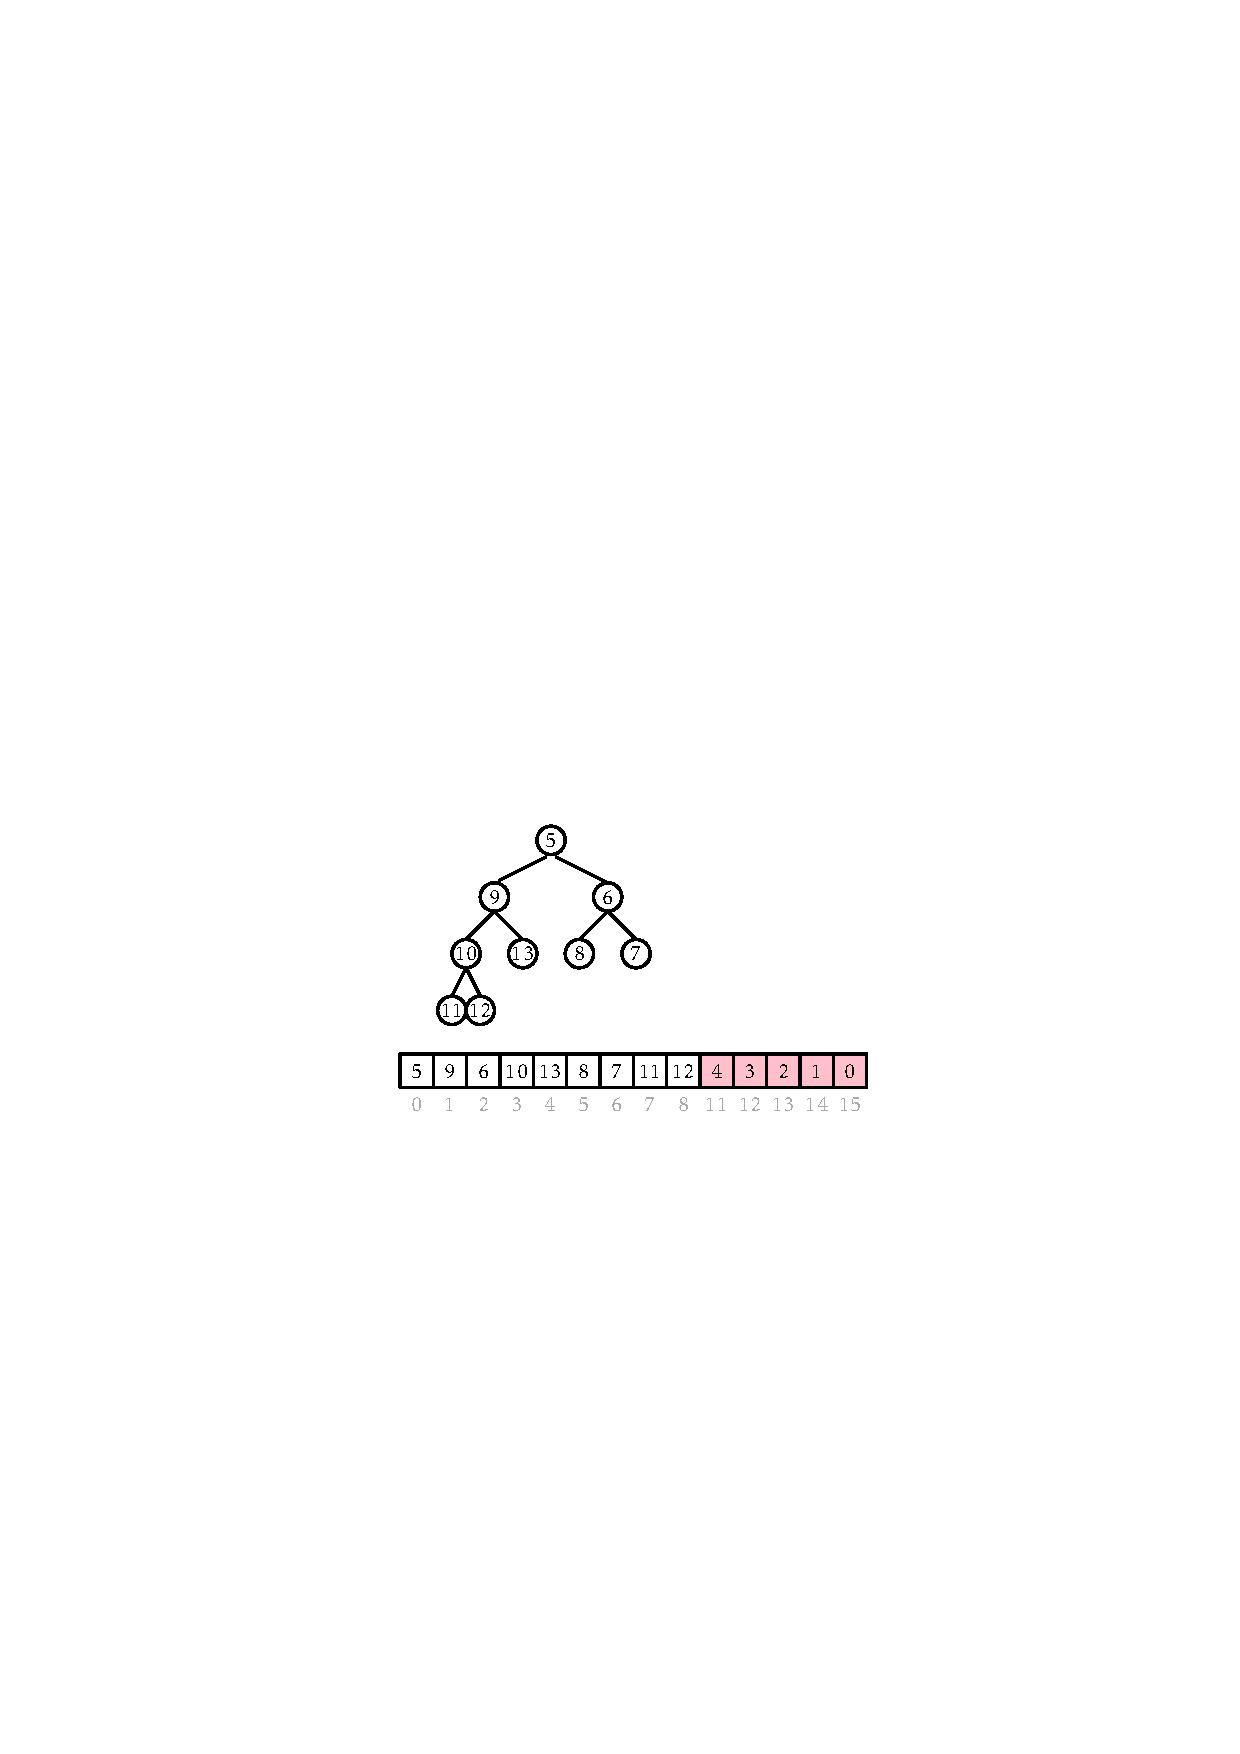
\includegraphics[scale=0.90909]{figs/heapsort}
  \end{center}
  \caption[Heap sort]{
  	Um instantâneo da execução de #heapSort(a,c)#. A parte sombreada da matriz já está classificada. A parte não sombreada é um #BinaryHeap#. Durante a próxima iteração, o elemento $5$ será colocado na posição do array $8$.}
  \figlabel{heapsort}
\end{figure}

\javaimport{ods/BinaryHeap.sort(a,c)}
\cppimport{ods/BinaryHeap.sort(b)}
\pcodeimport{ods/Algorithms.heapSort(a)}

Uma sub-rotina chave no tipo heap é o construtor para transformar um array não ordenado #a# em uma pilha. Seria fácil fazer isso em um tempo$O(#n#\log#n#)$ chamando repetidamente o método de #BinaryHeap# #add(x)#, mas podemos fazer melhor usando um algoritmo que execute de baixo para cima. Lembre-se de que, em uma pilha binária, os filhos de #a[i]# são armazenados nas posições #a[2i+1]# e #a[2i+2]#. Isso implica que os elementos $#a#[\lfloor#n#/2\rfloor],\ldots,#a[n-1]# $ não têm filhos. Em outras palavras, cada um de $#a#[\lfloor#n#/2\rfloor],\ldots,#a[n-1]# $ é um sub-heap de tamanho 1. Agora, trabalhando para trás, podemos chamar #trickleDown(i)# para cada $#i#\in\{\lfloor#n#/2\rfloor-1,\ldots,0\}$. Isso funciona, porque no momento em que chamamos #trickleDown(i)#, cada um dos dois filhos de #a[i]# são a raiz de um sub-heap, então, chamar #trickleDown(i)# faz #a[i]# a raiz do seu próprio sub-heap.
\javaimport{ods/BinaryHeap.BinaryHeap(a,c)}
\cppimport{ods/BinaryHeap.BinaryHeap(b)}

O interessante desta estratégia de baixo para cima é que é mais eficiente do que chamar #add(x)# #n# vezes. Para ver isso, observe que, para $#n#/2$ elementos, não fazemos nenhum trabalho, para $#n#/4$ elementos, chamamos #trickleDown(i)# em um sub-heap enraizado em #a[i]# e cuja altura é um, para $#n#/8$ elementos, chamamos #trickleDown(i)# em um subheap cuja altura é dois e assim por diante. Uma vez que o trabalho realizado por #trickleDown(i)# é proporcional à altura do sub-heap enraizado em #a[i]#, isso significa que o trabalho total feito é no máximo
\[
    \sum_{i=1}^{\log#n#} O((i-1)#n#/2^{i})
    \le \sum_{i=1}^{\infty} O(i#n#/2^{i})
    = O(#n#)\sum_{i=1}^{\infty} i/2^{i}
    =  O(2#n#) = O(#n#) \enspace .
\]
A segunda e última igualdade deriva do reconhecimento que a soma 
$\sum_{i=1}^{\infty} i/2^{i}$ é igual, por definição do valor esperado, ao número esperado de vezes que lançamos uma moeda e incluindo a primeira vez que a moeda aparece como cara e aplicando \lemref{coin-tosses}.

O seguinte teorema descreve o desempenho de #heapSort(a,c)#.
\begin{thm}
  O método #heapSort(a,c)# executa em um tempo $O(#n#\log #n#)$ e realiza no máximo $2#n#\log #n# + O(#n#)$ comparações.
\end{thm}

\begin{proof}
	O algoritmo é executado em três etapas: (1)~transformando #a# em um heap, (2)~extraindo repetidamente o elemento mínimo de #a# e (3)~revertendo os elementos em #a#. Nós apenas argumentamos que o passo~1 leva um tempo $O(#n#)$ e executa $O(#n#)$ comparações. O Passo~3 leva um tempo $O(#n#)$ e não realiza comparações. O passo~2 executa #n# chamadas para #trickleDown(0)#. A $i$-ésima chamada ocorre em um heap de tamanho $#n#-i$ e executa no máximo $2\log(#n#-i)$ comparações. Somando isso sobre $i$ dá
\[
   \sum_{i=0}^{#n#-i} 2\log(#n#-i) 
   \le \sum_{i=0}^{#n#-i} 2\log #n#
   =  2#n#\log #n#
\]
Adicionando o número de comparações realizadas em cada uma das três etapas completa a prova.
\end{proof}

\subsection{Um Limite Inferior para classificação baseada em comparação}

\index{limite lnferior}%
\index{limite lnferior para ordenação}%
Nós já vimos três algoritmos de classificação baseados em comparação que executam cada um em um tempo $O(#n#\log #n#)$. Agora devemos estar pensando se existem algoritmos mais rápidos. A resposta curta a esta pergunta é não. Se as únicas operações permitidas nos elementos de #a# são comparações, nenhum algoritmo pode evitar fazer $#n#\log #n#$ comparações. Isso não é difícil de provar, mas requer um pouco de imaginação. Em última análise, decorre do fato de que
\[
   \log(#n#!) 
     = \log #n# + \log (#n#-1) + \dots + \log(1) 
     = #n#\log #n# - O(#n#)
    \enspace .
\]
(Provar este fato é deixado para o \excref{log-factorial}.)

Começaremos concentrando nossa atenção em algoritmos determinísticos como merge-sort e heap-sort e em um valor fixo particular de #n#. Imagine que esse algoritmo está sendo usado para classificar #n# elementos distintos. A chave para provar o limite inferior é observar que, para um algoritmo determinístico com um valor fixo de #n#, o primeiro par de elementos que são comparados é sempre o mesmo. Por exemplo, em #heapSort(a,c)#, quando #n# é igual, a primeira chamada para #trickleDown(i)# é com #i=n/2-1# e a primeira comparação é entre os elementos #a[n/2-1]# e #a[n-1]#.

Uma vez que todos os elementos de entrada são distintos, esta primeira comparação tem apenas dois possíveis resultados. A segunda comparação feita pelo algoritmo pode depender do resultado da primeira comparação. A terceira comparação pode depender dos resultados dos dois primeiros, e assim por diante. Desta forma, qualquer algoritmo de classificação determinística baseado em comparação pode ser visto como uma árvore \emph{árvore de comparação} enraizada.
\index{arvore@árvore de comparação}%
Cada nó interno, #u#, desta árvore é rotulado com um par de índices #u.i# e #u.j#. Se $#a[u.i]#<#a[u.j]#$ o algoritmo prossegue para a subárvore esquerda, caso contrário, ele passa para a subárvore direita. Cada folha #w# desta árvore é rotulada com uma permutação $#w.p[0]#,\ldots,#w.p[n-1]#$ de $0,\ldots,#n#-1$. Essa permutação representa aquele que é necessário para classificar #a# se a árvore de comparação chegar a esta folha. Isso é,
\[
   #a[w.p[0]]#<#a[w.p[1]]#<\cdots<#a[w.p[n-1]]# \enspace .
\]
Um exemplo de uma árvore de comparação para um array de tamanho #n=3# é mostrado em
\figref{comparison-tree}.
\begin{figure}
  \begin{center}
    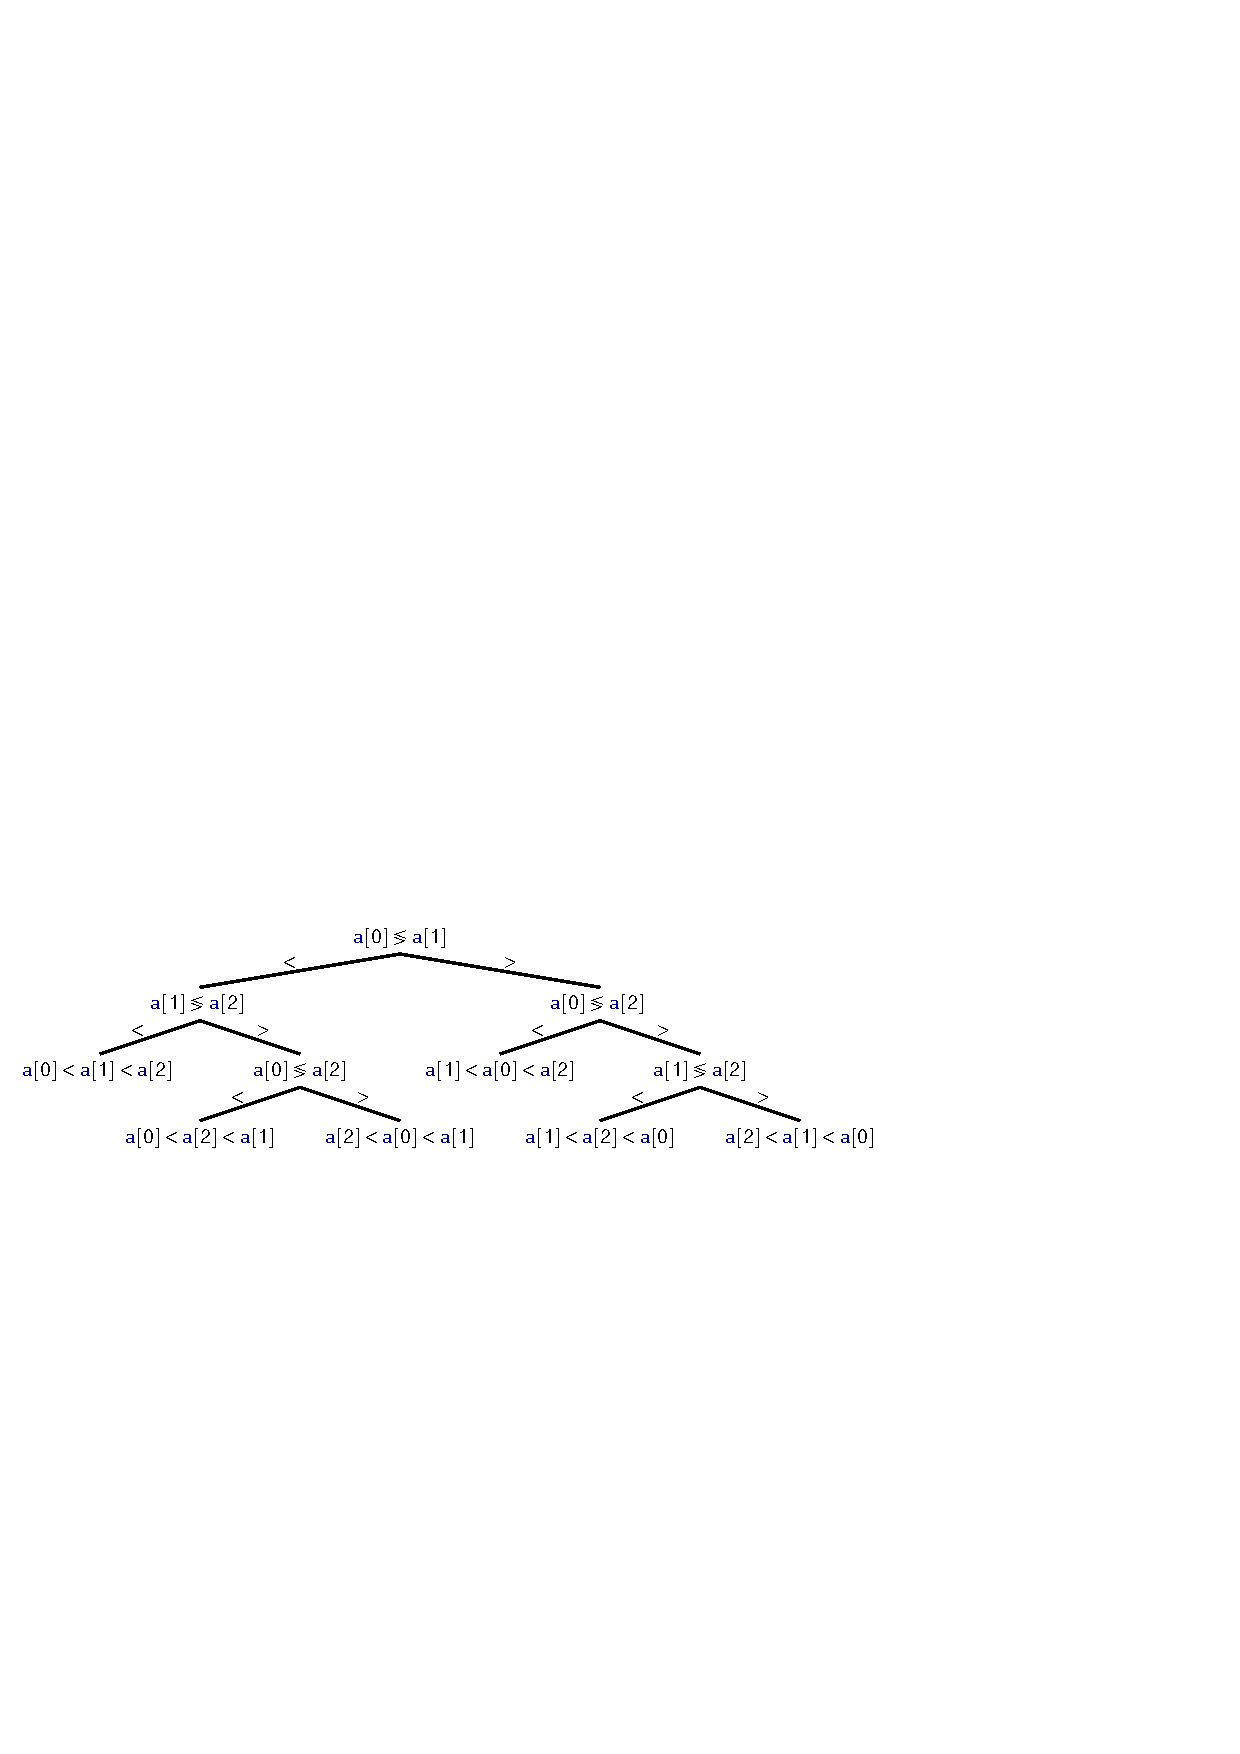
\includegraphics[width=\ScaleIfNeeded]{figs/comparison-tree}
  \end{center}
  \caption[Uma árvore de comparação]{Uma árvore de comparação para ordenar um array $#a[0]#,#a[1]#,#a[2]#$ de tamanho #n=3#.}
  \figlabel{comparison-tree}
\end{figure}

A árvore de comparação para um algoritmo de classificação nos diz tudo sobre o algoritmo. Ele nos diz exatamente a sequência de comparações que será realizada para qualquer matriz de entrada, #a#, tendo #n# elementos distintos e nos diz como o algoritmo irá reordenar #a# para ordená-lo. Consequentemente, a árvore de comparação deve ter pelo menos $#n#!$ folhas; se não, então há duas permutações distintas que levam à mesma folha; portanto, o algoritmo não classifica corretamente pelo menos uma dessas permutações.

Por exemplo, a árvore de comparação em \figref{comparison-tree-2} tem apenas $4<3!=6$ folhas. Inspecionando esta árvore, vemos que os dois arrays de entrada $3,1,2$ e $3,2,1 $ ambos levam à folha mais à direita. Na entrada $3,1,2$, esta folha corretamente exibe $#a[1]#=1,#a[2]#=2,#a[0]#=3$. No entanto, na entrada $3,2,1$, este nó incorretamente fornece $#a[1]#=2,#a[2]#=1,#a[0]#=3$. Esta discussão leva ao limite inferior primário para algoritmos baseados em comparação.

\begin{figure}
  \begin{center}
    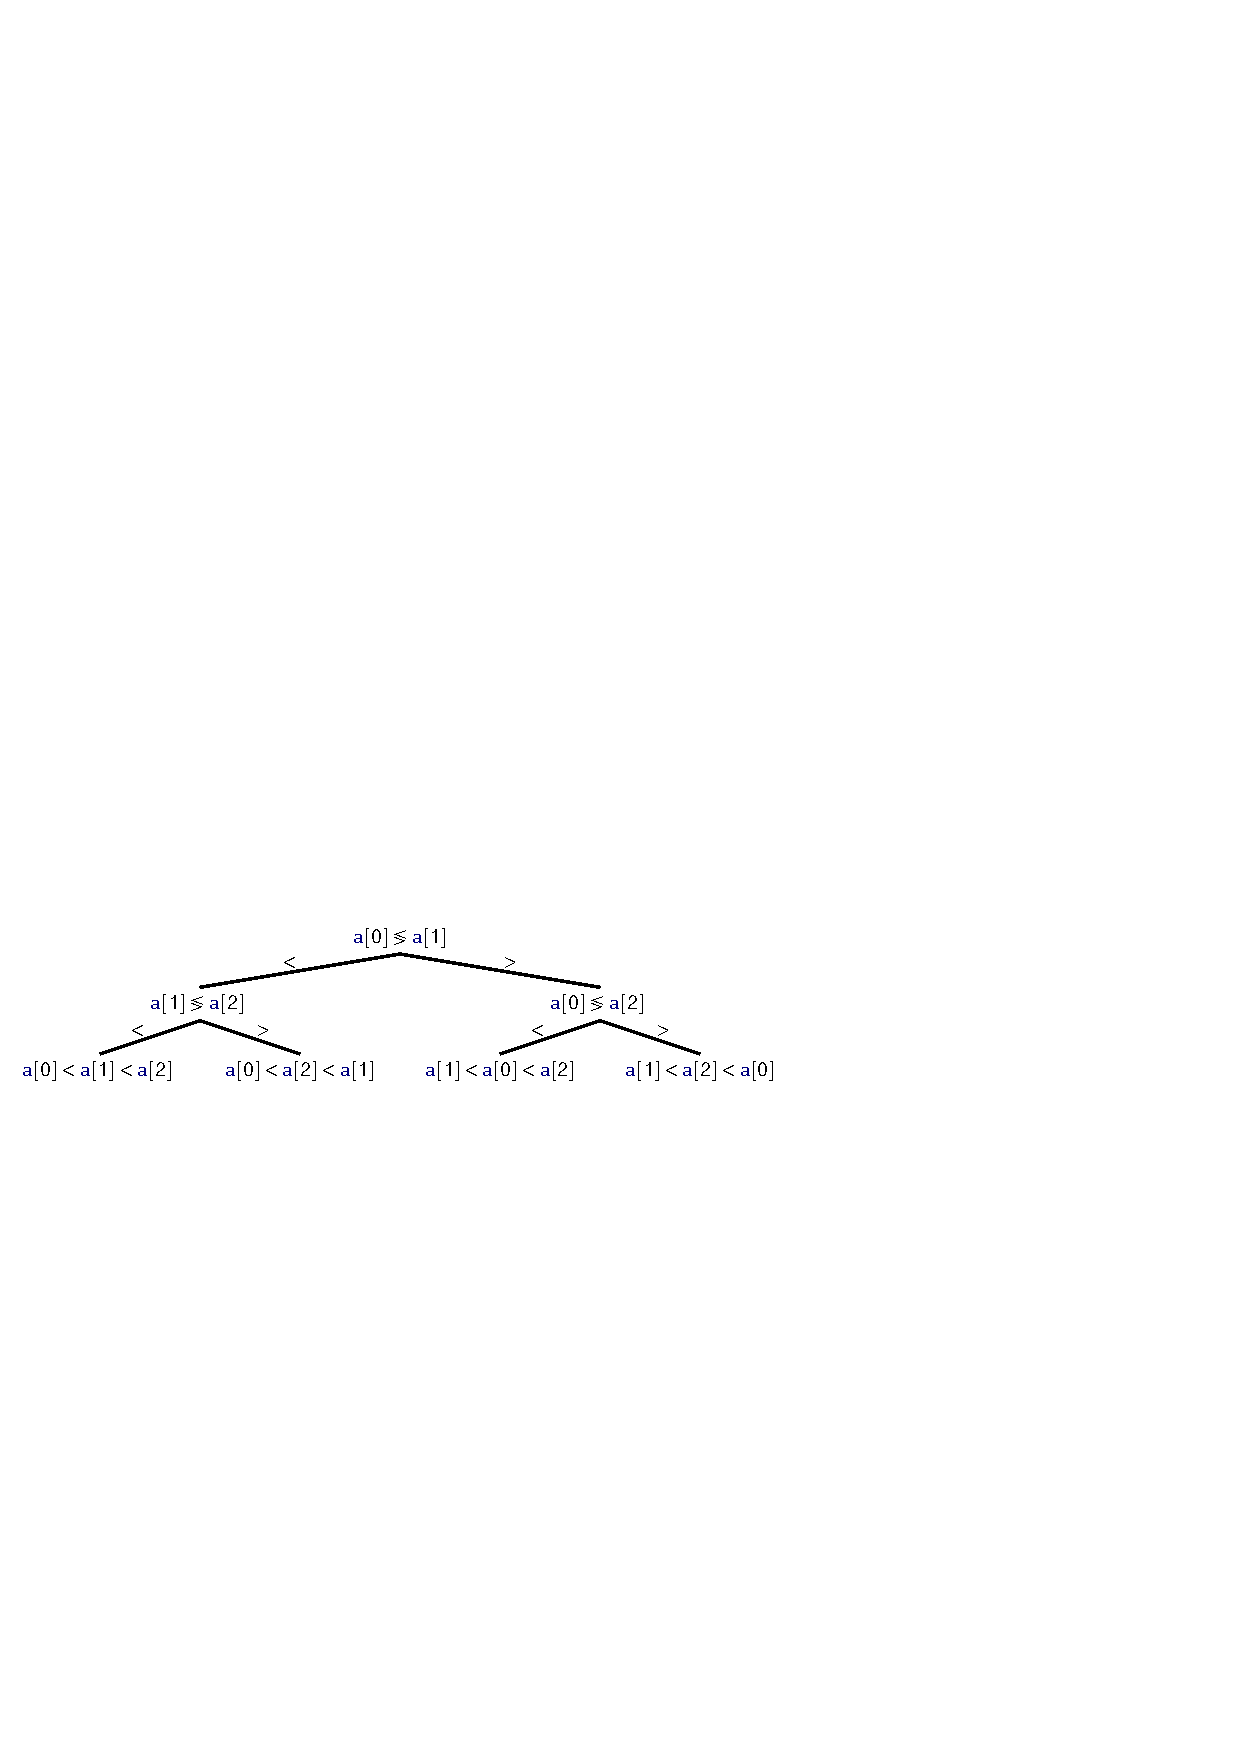
\includegraphics[width=\ScaleIfNeeded]{figs/comparison-tree-b}
  \end{center}
  \caption{Uma árvore de comparação que não classifica corretamente todas as permutações de entrada.}
  \figlabel{comparison-tree-2}
\end{figure}

\begin{thm}\thmlabel{deterministic-sorting-lower-bound}
	Para qualquer algoritmo de classificação baseado em comparação determinística $\mathcal{A}$ e qualquer inteiro $#n#\ge1$, existe um array de entrada #a# de comprimento #n# tal que $\mathcal{A}$ executa em menos $\log(#n#!)=#n#\log#n#-O(#n#)$ comparações ao classificar #a#.
\end{thm}

\begin{proof}
	Na discussão anterior, a árvore de comparação definida por $\mathcal{A}$ deve ter pelo menos $#n#!$ folhas. Uma prova indutiva fácil mostra que qualquer árvore binária com $k$ folhas tem uma altura de pelo menos $\log k$. Portanto, a árvore de comparação para $\mathcal{A}$ tem uma folha, #w#, com uma profundidade de pelo menos $\log(#n#!)$ e existe um array de entrada #a# que leva a esta folha. O array de entrada #a# é uma entrada para a qual $\mathcal{A}$ faz pelo menos $\log(#n#!)$ comparações.
\end{proof}

\thmref{deterministic-sorting-lower-bound} trata de algoritmos determinísticos, como o merge-sort e o heap-sort, mas não nos conta nada sobre algoritmos randomizados como quicksort. Poderia um algoritmo randomizado vencer o limite inferior $\log(#n#!)$ no número de comparações? A resposta, novamente, é não. Novamente, a maneira de provar isso é pensar de forma diferente sobre o que é um algoritmo randomizado.

Na discussão a seguir, assumiremos que nossas árvores de decisão foram "limpas" da seguinte maneira: qualquer nó que não pode ser alcançado por algum array de entrada #a# é removido. Esta limpeza implica que a árvore tem exatamente $#n#!$ folhas. Tem pelo menos $#n#!$ folhas porque, caso contrário, não conseguiria ordenar corretamente. Tem no máximo $#n#!$ folhas desde que cada uma das possíveis $#n#!$ permutações de #n# elementos distintos seguem exatamente uma raiz para o caminho da folha na árvore de decisão.

Podemos pensar em um algoritmo de classificação aleatorizado, $\mathcal{R}$, como um algoritmo determinista que leva duas entradas: o array de entrada #a# que deve ser ordenado e uma sequência longa $b=b_1,b_2,b_3,\ldots,b_m$ de números reais aleatórios no intervalo $[0,1]$. Os números aleatórios fornecem a randomização para o algoritmo. Quando o algoritmo quer jogar uma moeda ou fazer uma escolha aleatória, ele faz isso usando algum elemento de $b$. Por exemplo, para calcular o índice do primeiro pivô no quicksort, o algoritmo pode usar a fórmula $\lfloor n b_1\rfloor$.

Agora, note que se nós fixamos $b$ em alguma sequência particular $\hat{b}$, então $\ mathcal{R}$ se torna um algoritmo de classificação determinista, $\mathcal{R}(\hat{b})$, que tem uma árvore de comparação associada, $\mathcal{T}(\hat {b})$. Em seguida, note que se selecionarmos #a# para ser uma permutação aleatória de $\{1,\ldots,#n#\}$, então isso é equivalente a selecionar uma folha aleatória, #w#, a partir de $#n#!$ folhas de $\mathcal{T}(\hat{b})$.

\excref{randomized-lower-bound} pede para provar isso, se selecionarmos uma folha aleatória de qualquer árvore binária com $k$ folhas, então a profundidade esperada dessa folha é pelo menos $\log k$. Portanto, o número esperado de comparações realizadas pelo algoritmo (determinístico) $\mathcal{R}(\hat{b})$ quando é dada um array de entrada contendo uma permutação aleatória de $\{1,\ldots,n\}$ é pelo menos $\log(#n#!)$. Finalmente, note que isso é verdade para todas as opções de $\hat{b}$, portanto, é válido para $\mathcal{R}$. Isso completa a prova do limite inferior para algoritmos randomizados.

\begin{thm}\thmlabel{randomized-sorting-lower-bound}
	Para qualquer inteiro $n\ge1$ e qualquer algoritmo de classificação baseado em comparação (determinístico ou randomizado) $\mathcal{A}$, o número esperado de comparações feito por $\mathcal{A}$ ao classificar uma permutação aleatória
  de $\{1,\ldots,n\}$ é de pelo menos $\log(#n#!) = #n#\log#n#-O(#n#)$.
\end{thm}



\section{Ordenação por Contagem e Ordenação Radix}

Nesta seção, estudamos dois algoritmos de classificação que não são baseados em comparação. Especializados para classificar inteiros pequenos, esses algoritmos evitam os limites inferiores de \thmref{deterministic-sorting-lower-bound} usando (partes de) os elementos em #a# como índices em um array.
Considere uma declaração da forma
\[
  #c[a[i]]# = 1 \enspace .
\]
Esta declaração é executada em tempo constante, mas tem #c.length# possíveis resultados diferentes, dependendo do valor de #a[i]#. Isso significa que a execução de um algoritmo que faz tal afirmação não pode ser modelada como uma árvore binária. Em última análise, essa é a razão pela qual os algoritmos nesta seção podem classificar mais rapidamente do que os algoritmos baseados em comparação.

\subsection{Ordenação por Contagem}

Suponhamos que tenhamos um array de entrada #a# consistindo de #n# inteiros, cada um no intervalo $0,\ldots,#k#-1$. O \emph{count-sort}
\index{ordenação por contagem}% 
algoritmo classifica #a# usando um array auxiliar #c# de contadores. Ele produz uma versão ordenada de #a# como um array auxiliar #b#.

A ideia por trás do tipo de contagem é simples: para cada $#i#\in\{0,\ldots,#k#-1\}$, conte o número de ocorrências de #i# em #a# e armazene isso em #c[i]#. Agora, após a classificação, a saída parecerá #c[0]# ocorrências de 0, seguido de #c[1]# ocorrências de 1, seguido de #c[2]# ocorrências de 2, \ldots, seguido de #c[k-1]# ocorrências de #k-1#. O código que faz isso é bem inteligente, e sua execução está ilustrada em
\figref{countingsort}:
\codeimport{ods/Algorithms.countingSort(a,k)}

\begin{figure}
  \begin{center}
    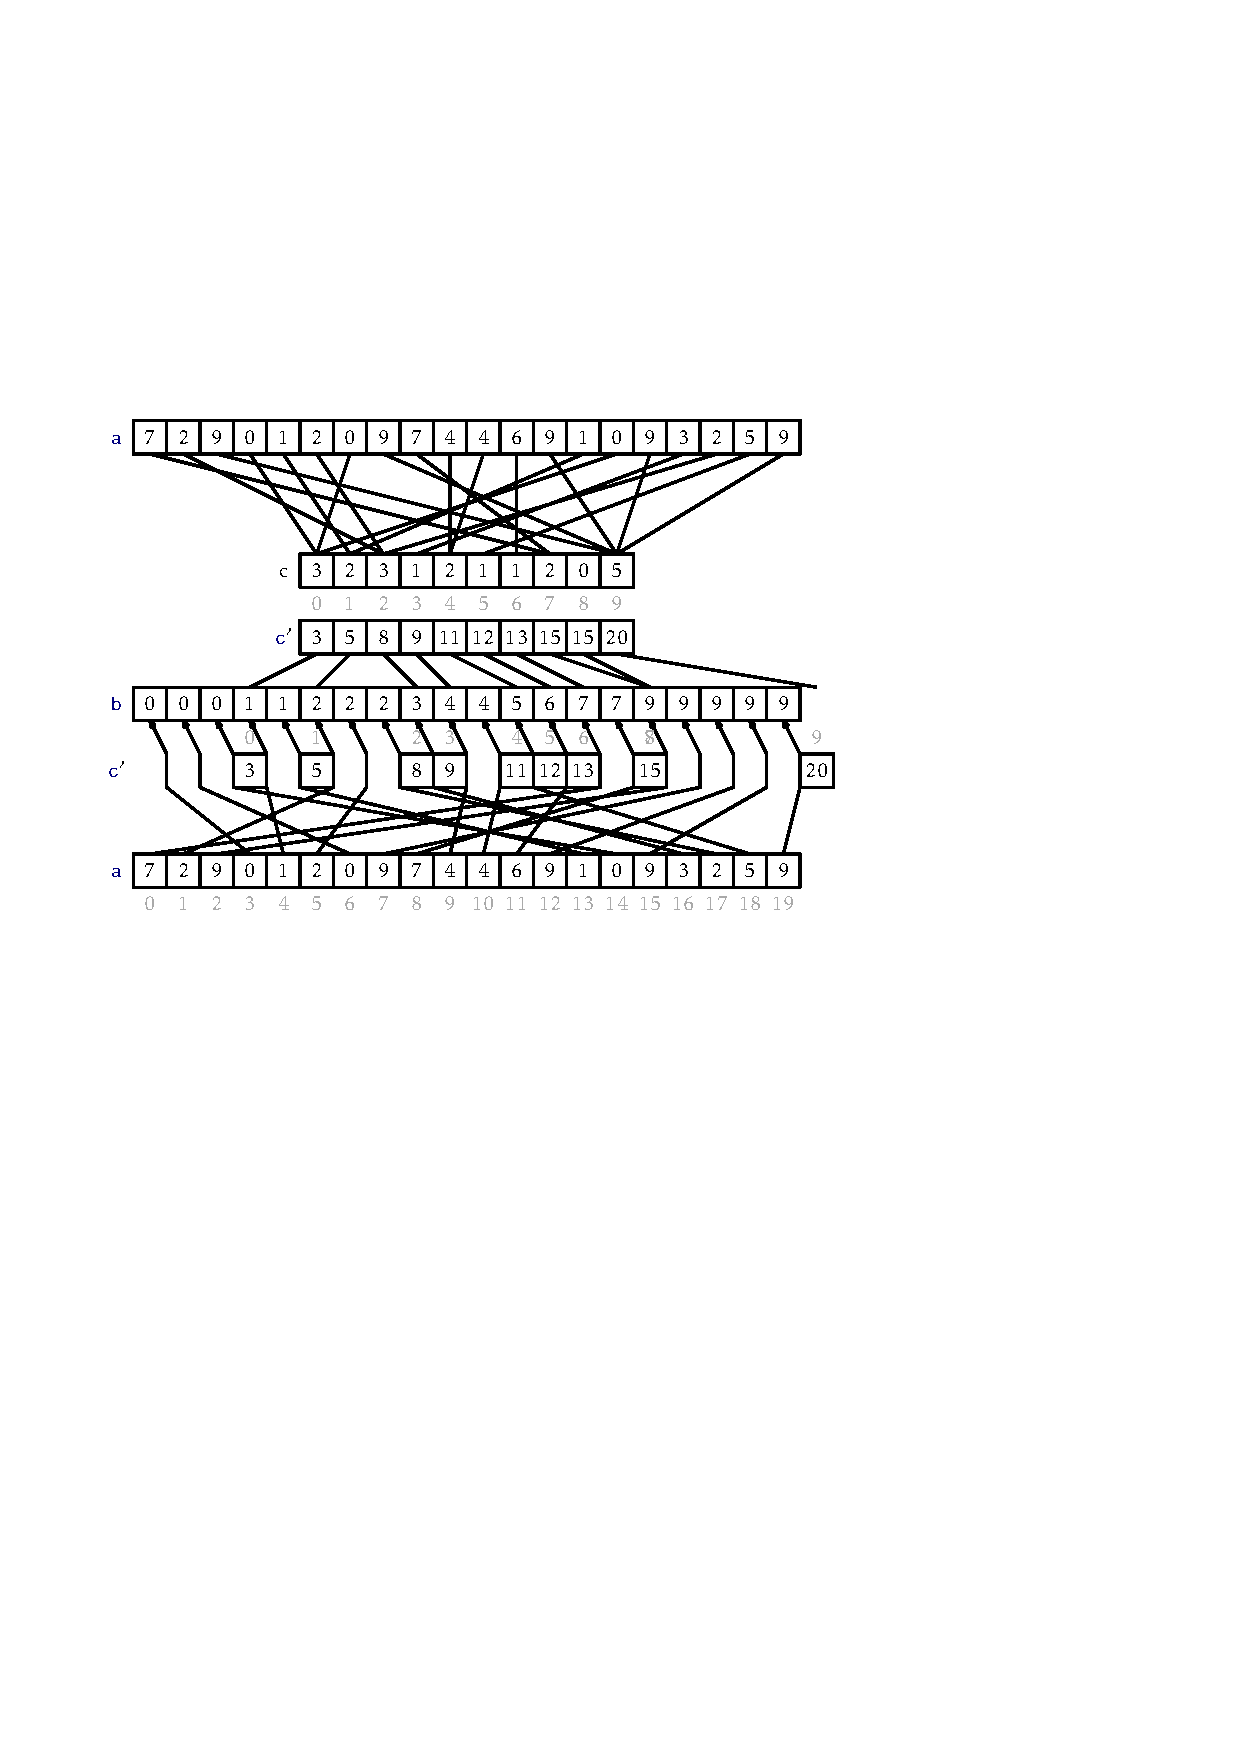
\includegraphics[width=\ScaleIfNeeded]{figs/countingsort}
  \end{center}
  \caption{A operação do tipo de contagem em um array de comprimento $#n#=20$ que armazena números inteiros $0,\ldots,#k#-1=9$.}
  \figlabel{countingsort}
\end{figure}

O primeiro loop #for# neste código define cada contador #c[i]# para que ele conte o número de ocorrências de #i# em #a#. Ao usar os valores de #a# como índices, esses contadores podem ser computados em um tempo $O(#n#)$ com um único loop \textit{for}. Neste ponto, poderíamos usar #c# para preencher o array de saída #b# diretamente. No entanto, isso não funcionaria se os elementos de #a# tiverem dados associados. Portanto, gastamos um pouco de esforço extra para copiar os elementos de #a# em #b#.

O próximo loop #for#, que leva um tempo $O(#k#)$, calcula uma soma dos contadores para que #c[i]# se torne o número de elementos em #a# que são menores ou iguais a #i#. Em particular, para cada $#i#\in\{0,\ldots,#k#-1\}$, o array de saída, #b#, terá
\[
   #b[c[i-1]]#=#b[c[i-1]+1]=#\cdots=#b[c[i]-1]#=#i# \enspace .
\]
Finalmente, o algoritmo varre #a# de trás para frente para colocar seus elementos, em ordem, em um array de saída #b#. Ao varrer, o elemento #a[i]=j# é colocado na posição #b[c[j]-1]# e o valor #c[j]# é decrementado.

\begin{thm}
	O método #countingSort(a,k)# pode classificar um array #a# contendo #n# inteiros no conjunto $\{0,\ldots,#k#-1\}$ em um tempo $O(#n#+#k#)$.
\end{thm}

O algoritmo de classificação de contagem tem a boa propriedade de ser \emph{estável};
\index{algoritmo de classificação estável}% 
preserva a ordem relativa de elementos iguais. Se dois elementos #a[i]# e #a[j]# tiverem o mesmo valor e $#i#<#j#$ então #a[i]# aparecerá antes #a[j]# em #b#. Isso será útil na próxima seção.

\subsection{Ordenação Radix}

A ordenação por contagem é muito eficiente para classificar um array de inteiros quando o comprimento, #n#, do array não é muito menor do que o valor máximo, $#k#-1$, que aparece no array. O algoritmo \emph{radix-sort}
\index{ordenação radix}%
, que descrevemos agora, usa várias passagens de ordenação por contagem para permitir uma gama muito maior de valores máximos.


A ordenação por radix classifica #w#-bit inteiros usando $#w#/#d#$ passos de ordenação por contagem para classificar esses números inteiros de #d# bits de cada vez. \footnote{Assumimos que #d# divide #w#, caso contrário nós sempre podemos aumentar #w# para $#d#\lceil #w#/#d#\rceil$.} Mais precisamente, a ordenação por  radix primeiro classifica os inteiros por seus #d# bits menos significativos, então os próximos #d# bits significativos e assim, até que, na última passagem, os números inteiros sejam classificados por seus #d# bits mais significativos. 
\codeimport{ods/Algorithms.radixSort(a)} 
(Neste código, a expressão #(a[i]>>d*p)&((1<<d)-1)# extrai o inteiro cuja representação binária é dado pelos bits
$(#p#+1)#d#-1,\ldots,#p##d#$ de #a[i]#.)
Um exemplo dos passos deste algoritmo é mostrado na \figref{radixsort}.

\begin{figure}
  \begin{center}
    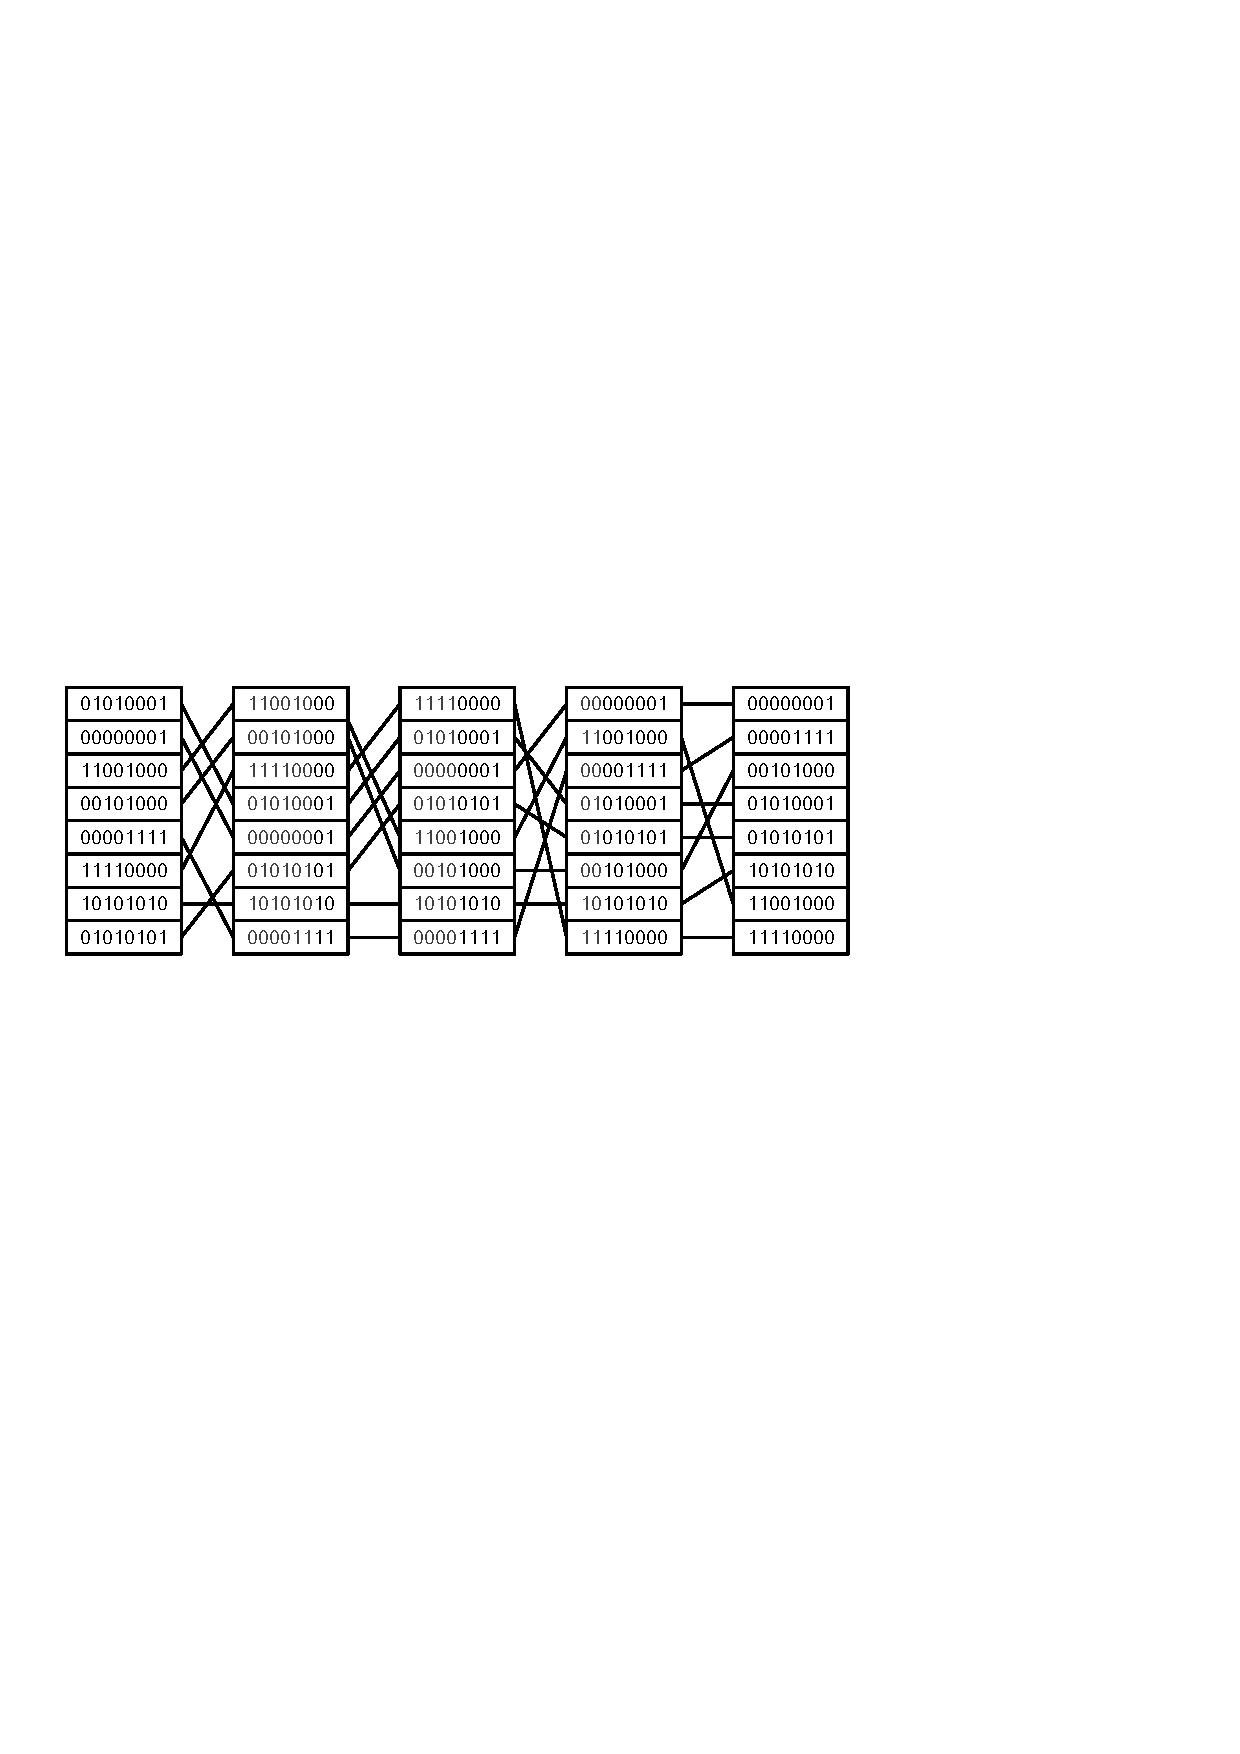
\includegraphics[width=\ScaleIfNeeded]{figs/radixsort}
  \end{center}
  \caption{Usando radixsort para ordenar inteiros de $#w#=8$-bits usando 4 passagens
   da ordenação por contagem com inteiros de $#d#=2$-bits.}
  \figlabel{radixsort}
\end{figure}

Este algoritmo notável classifica corretamente porque o tipo de contagem é um algoritmo de classificação estável. Se $#x#<#y#$ para dois elementos de #a#, e o bit mais significativo em que #x# difere de #y# tenha índice $r$, então #x# será colocado antes de #y# durante o passo $\lfloor r/#d#\rfloor$ e as passagens subsequentes não alterarão a ordem relativa de #x# e #y#.

Radix-sort executa #w/d# passos de ordenação por contagem. Cada passagem requer um tempo $O(#n#+2^{#d#})$. Portanto, o desempenho da ordenação por radix é dado pelo seguinte teorema.
\begin{thm}\thmlabel{radix-sort}
	Para qualquer inteiro $#d#>0$, o método #radixSort(a,k)# pode classificar um array #a# contendo #n# inteiros de #w#-bits em um tempo $O((#w#/#d#)(#n#+2^{#d#}))$.
\end{thm}

Se pensarmos, em vez disso, que os elementos do array estão no intervalo $\{0,\ldots,#n#^c-1\}$ e pegarmos $#d#=\lceil\log#n#\rceil$ obtemos a seguinte versão de \thmref{radix-sort}.
\begin{cor}\corlabel{radix-sort-poly}
	O método #radixSort(a,k)# pode classificar um array #a# contendo #n# valores inteiros na faixa $\{0,\ldots,#n#^c-1\}$ em um tempo $O(c#n#)$.
\end{cor}

\section{Discussão e Exercícios}

A classificação é \emph{o} problema algorítmico fundamental na ciência da computação, e tem uma longa história. Knuth \cite{k97v3} atribui o algoritmo de classificação de mesclagem a von~Neumann (1945). Quicksort é devido a Hoare \cite{h61}. O algoritmo de classificação de heap original é devido a Williams \cite{w64}, mas a versão apresentada aqui (em que o heap é construído de baixo para cima em um tempo $O(#n#)$) é devido a Floyd \cite{f64}. Os limites inferiores para a classificação baseada em comparação parecem ser folclore. A tabela a seguir resume o desempenho desses algoritmos baseados em comparação:

\begin{center}
  \begin{tabular}{|l|r@{}l@{ }l|l|} \hline
      & \multicolumn{3}{c|}{comparações} & no local  \\ \hline
    Merge-sort & $#n#\log #n#$ & &  pior caso & Não  \\
    Quicksort & $1.38#n#\log #n#$ & ${}+ O(#n#)$ & esperado & Sim \\
    Heap-sort & $2#n#\log #n#$ & ${}+ O(#n#)$ & pior caso & Sim \\ \hline
  \end{tabular}
\end{center}

Cada um desses algoritmos baseados em comparação tem suas vantagens e desvantagens. Merge-sort tem o menor número de comparações e não depende da randomização. Infelizmente, ele usa um array auxiliar durante a fase de mesclagem. Alocar este array pode ser caro e é um ponto potencial de falha se a memória for limitada. Quicksort é um algoritmo \emph{no local}
\index{algoritmo no local}%% 
e é o segundo próximo em termos de número de comparações, mas é randomizado, portanto, este tempo de execução nem sempre é garantido. 
Heap-sort faz o maior número de comparações, mas é no local e determinístico.

Existe uma configuração na qual a ordenação por merge é um vencedor claro; isso ocorre ao ordenar uma lista encadeada. Nesse caso, o array  auxiliar não é necessário; duas listas encadeadas ordenadas são facilmente incorporadas em uma única lista ordenada por manipulação de ponteiro (veja \excref{list-merge-sort}).

Os algoritmos de classificação de contagem e classificação de radix aqui descritos são devidos a Seward \cite[Seção~2.4.6]{s54}. No entanto, variantes de radix-sort foram utilizadas desde a década de 1920 para classificar os cartões de perfuração usando máquinas de classificação de cartão perfurado. Essas máquinas podem classificar uma pilha de cartões em duas pilhas com base na existência (ou não) de um buraco em um local específico no cartão. Repetir este processo para diferentes locais de furos dá uma implementação de tipo radix.

Finalmente, observamos que a ordenação por contagem e a ordenação por radix podem
ser usadas para classificar outros tipos de números além de números inteiros não
negativos. Modificações diretas da ordenação por contagem podem classificar inteiros, em qualquer intervalo $\{a,\ldots,b\}$, em $O(#n#+b-a)$. 
Da mesma forma, a ordenação por radix pode classificar inteiros no mesmo intervalo em um tempo $O(#n#(\log_{#n#}(ba))$. 
Finalmente, esses dois algoritmos também podem ser usados para classificar
números de ponto flutuante no Formato de ponto flutuante IEEE 754.
Isso ocorre porque o formato IEEE foi projetado para permitir a comparação de dois números de ponto flutuante comparando seus valores como se fossem inteiros em uma representação binária de sinal-magnitude \cite{ieee754}.
	
\begin{exc}
	Ilustre a execução de merge-sort e heap-sort em um array de entrada contendo $1,7,4,6,2,8,3,5$. Dê uma amostra que ilustre uma possível execução de quicksort no mesmo array.
\end{exc}

\begin{exc}\exclabel{list-merge-sort}
	Implementar uma versão do algoritmo de classificação por merge que ordena uma #DLList# sem usar um array auxiliar. (Veja \excref{dllist-sort}.)
\end{exc}

\begin{exc}
	Algumas implementações de #quickSort(a,i,n,c)# sempre usam #a[i]# como um pivô. Dê um exemplo de um array de entrada de comprimento #n# no qual tal implementação executaria $\binom{#n#}{2}$ comparações.
\end{exc}

\begin{exc}
	Algumas implementações de #quickSort(a,i,n,c)# sempre usam #a[i+n/2]# como um pivô. Forneça um exemplo de um array de entrada de comprimento #n# na qual tal implementação executaria $\binom{#n#}{2}$ comparações.
\end{exc}

\begin{exc}
	Mostre que, para qualquer implementação de #quickSort(a,i,n,c)# que escolha um pivô de forma determinística, sem primeiro olhar para qualquer valor em $#a[i]#,\ldots,#a[i+n-1]#$, existe um array de entrada de comprimento #n# que faz com que esta implementação realize $\binom{#n#}{2}$ comparações.
\end{exc}

\begin{exc}
	Crie um #Comparador#, #c#, que você poderia passar como um argumento para #quickSort(a,i,n,c)# e isso faria que o quicksort execute $\binom{#n#}{2}$ comparações. (Sugestão: o seu comparador na verdade não precisa analisar os valores que estão sendo comparados).
\end{exc}

\begin{exc}
	Analise o número esperado de comparações feitas pelo Quicksort um pouco mais cuidadosamente do que a prova de \thmref{quicksort}. Em particular, mostre que o número esperado de comparações é $2#n#H_#n# -#n# + H_#n#$.
\end{exc}

\begin{exc}
	Descreva um array de entrada que faz com que a ordenação heap realize pelo menos $2#n#\log #n#-O(#n#)$ comparações. Justifique sua resposta.
\end{exc}

\javaonly{
\begin{exc}
	A implementação de classificação de heap descrita aqui classifica os elementos na ordem ordenada reversa e, em seguida, inverte o array. Este último passo poderia ser evitado definindo um novo #Comparador# que anule os resultados da entrada #Comparador#, #c#. Explique por que isso não seria uma boa otimização. (Sugestão: considere o número de negações que devem ser feitas em relação ao tempo que leva para reverter o array).
\end{exc}
}

\begin{exc}
	Encontre outro par de permutações de $1,2,3$ que não sejam ordenados corretamente pela árvore de comparação em \figref{comparison-tree-2}.
\end{exc}

\begin{exc}\exclabel{log-factorial}
  Prove que $\log #n#! = #n#\log #n#-O(#n#)$.
\end{exc}

\begin{exc}
	Prove que uma árvore binária com $k$ folhas tem altura de pelo menos $\log k$.
\end{exc}

\begin{exc}\exclabel{randomized-lower-bound}
	Prove que, se escolhermos uma folha aleatória de uma árvore binária com $k$ folhas, a altura esperada desta folha é de pelo menos $\log k$.
% (Dica: Use a indução junto com a desigualdade $(k_1/k)\log k_1 +
%  (k_2/k)\log k_2) \ge  \log k-1$, quando $k_1+k_2=k$.)
\end{exc}

%Este foi um exercício estúpido, uma vez que os números de ponto flutuante IEEE 754 
%são ordenados corretamente quando são tratados como inteiros de 
%sinal-magnitude [isto é, um bit de sinal seguido por um número inteiro]
%\begin{exc}
%Os números de ponto flutuante simples são números da forma $x\cdot10^{y}$, onde
% $0\le x\le 1$ e $y$ é um número inteiro e cada $x$ e $y$ podem ser representados
% por mais $k$ bits. Descreva uma versão da ordenação por radix que possa ser usada
% para ordenar números de ponto flutuante simples.
%
%Estenda sua versão da ordenação por radix para que ele possa lidar com valores
% sinalizados de $x$ e $y$ e implemente uma versão da ordenação por radix que
% classifica os arrays tipo #flutuante#.
%\end{exc}

\begin{exc}
	A implementação de #radixSort(a,k)# fornecida aqui funciona quando o array de entrada, #a# contém apenas inteiros \cpponly{unsigned}\javaonly{non-negative}. \javaonly{Estenda esta implementação para que ela também funcione corretamente quando #a# contém números inteiros negativos e não negativos.} \cpponly{Escreva uma versão que funcione corretamente para inteiros sinalizados.}
\end{exc}

